
\documentclass[conference]{IEEEtran}

%\usepackage{polski} 
%\usepackage[utf8]{inputenc}

% *** MISC UTILITY PACKAGES ***
%
%\usepackage{ifpdf}
% Heiko Oberdiek's ifpdf.sty is very useful if you need conditional
% compilation based on whether the output is pdf or dvi.
% usage:
% \ifpdf
%   % pdf code
% \else
%   % dvi code
% \fi
% The latest version of ifpdf.sty can be obtained from:
% http://www.ctan.org/pkg/ifpdf
% Also, note that IEEEtran.cls V1.7 and later provides a builtin
% \ifCLASSINFOpdf conditional that works the same way.
% When switching from latex to pdflatex and vice-versa, the compiler may
% have to be run twice to clear warning/error messages.




% *** CITATION PACKAGES ***
%
%\usepackage{cite}
% cite.sty was written by Donald Arseneau
% V1.6 and later of IEEEtran pre-defines the format of the cite.sty package
% \cite{} output to follow that of the IEEE. Loading the cite package will
% result in citation numbers being automatically sorted and properly
% "compressed/ranged". e.g., [1], [9], [2], [7], [5], [6] without using
% cite.sty will become [1], [2], [5]--[7], [9] using cite.sty. cite.sty's
% \cite will automatically add leading space, if needed. Use cite.sty's
% noadjust option (cite.sty V3.8 and later) if you want to turn this off
% such as if a citation ever needs to be enclosed in parenthesis.
% cite.sty is already installed on most LaTeX systems. Be sure and use
% version 5.0 (2009-03-20) and later if using hyperref.sty.
% The latest version can be obtained at:
% http://www.ctan.org/pkg/cite
% The documentation is contained in the cite.sty file itself.



\usepackage{amsmath}
\newcommand{\beq}{\begin{equation}}
\newcommand{\eeq}{\end{equation}}
\newcommand{\sms}{\smallskip}
\newcommand{\ms}{\medskip}
\newcommand{\bs}{\bigskip}
\newcommand{\norm}[1]{\left\lVert#1\right\rVert}
\newtheorem{problem}{Problem}
\newtheorem{theorem}{Theorem}
\usepackage{graphicx}


% *** SPECIALIZED LIST PACKAGES ***
%
%\usepackage{algorithmic}
% algorithmic.sty was written by Peter Williams and Rogerio Brito.
% This package provides an algorithmic environment fo describing algorithms.
% You can use the algorithmic environment in-text or within a figure
% environment to provide for a floating algorithm. Do NOT use the algorithm
% floating environment provided by algorithm.sty (by the same authors) or
% algorithm2e.sty (by Christophe Fiorio) as the IEEE does not use dedicated
% algorithm float types and packages that provide these will not provide
% correct IEEE style captions. The latest version and documentation of
% algorithmic.sty can be obtained at:
% http://www.ctan.org/pkg/algorithms
% Also of interest may be the (relatively newer and more customizable)
% algorithmicx.sty package by Szasz Janos:
% http://www.ctan.org/pkg/algorithmicx






% correct bad hyphenation here
\hyphenation{op-tical net-works semi-conduc-tor}


\begin{document}

\title{Novel method of informative frequency band selection for vibration signal using Nonnegative Matrix Factorization of Short-Time Fourier Transform}


% author names and affiliations
% use a multiple column layout for up to three different
% affiliations
% \author{\IEEEauthorblockN{Michael Shell}
% \IEEEauthorblockA{School of Electrical and\\Computer Engineering\\
% Georgia Institute of Technology\\
% Atlanta, Georgia 30332--0250\\
% Email: http://www.michaelshell.org/contact.html}
% \and
% \IEEEauthorblockN{Homer Simpson}
% \IEEEauthorblockA{Twentieth Century Fox\\
% Springfield, USA\\
% Email: homer@thesimpsons.com}
% \and
% \IEEEauthorblockN{James Kirk\\ and Montgomery Scott}
% \IEEEauthorblockA{Starfleet Academy\\
% San Francisco, California 96678--2391\\
% Telephone: (800) 555--1212\\
% Fax: (888) 555--1212}}

% conference papers do not typically use \thanks and this command
% is locked out in conference mode. If really needed, such as for
% the acknowledgment of grants, issue a \IEEEoverridecommandlockouts
% after \documentclass

% for over three affiliations, or if they all won't fit within the width
% of the page, use this alternative format:
% 
\author{\IEEEauthorblockN{Jacek Wodecki\IEEEauthorrefmark{1},
Piotr Kruczek\IEEEauthorrefmark{1},
Anna Bartkowiak\IEEEauthorrefmark{2}, 
Rados{\l}aw Zimroz\IEEEauthorrefmark{3} and
Agnieszka Wy{\l}oma{\'n}ska\IEEEauthorrefmark{1}}
\IEEEauthorblockA{\IEEEauthorrefmark{1}KGHM CUPRUM Ltd CBR, 53-659 Wroc{\l}aw, Poland}
\IEEEauthorblockA{\IEEEauthorrefmark{2}Institute of Computer Science, Wroc{\l}aw University, 50-383 Wroc{\l}aw, Poland, retired}
\IEEEauthorblockA{\IEEEauthorrefmark{3}Diagnostics and Vibro-Acoustics Science Laboratory,\\
Wroc{\l}aw University of Science and Technology, Wroc{\l}aw, Poland}}



% use for special paper notices
% \IEEEspecialpapernotice{(Invited Paper)}

% make the title area
\maketitle

% As a general rule, do not put math, special symbols or citations
% in the abstract
\begin{abstract}
The problem of local damage detection in rotating machines is currently the highly important subject of interest. In the literature one can find many different strategies. One of the most common approaches is the vibration signal analysis aiming at informative frequency band selection. In case of simply structured signals classic methods (e.g. spectral kurtosis) are sufficient and return clear information about the damage. However, in real-world cases the signal is usually much more complicated. Indeed, such signals consist of many different components, for instance: damage-related cyclic impulses, high energy non-cyclic impulses not related to damage or heavy-tailed background noise etc. Hence, there is a growing need for robust damage detection methods. In this paper a novel method of informative frequency band selection is proposed. It utilizes the approach of Non-negative Matrix Factorization applied to time-frequency signal representation. The described algorithm is evaluated using simulated signal containing several different components, that resembles real-life vibration signal from copper ore crusher. Using the obtained structure of informative frequency band it is possible to filter particular components out of the original signal.
\end{abstract}

% no keywords




% For peer review papers, you can put extra information on the cover
% page as needed:
% \ifCLASSOPTIONpeerreview
% \begin{center} \bfseries EDICS Category: 3-BBND \end{center}
% \fi
%
% For peerreview papers, this IEEEtran command inserts a page break and
% creates the second title. It will be ignored for other modes.
\IEEEpeerreviewmaketitle



\section{Introduction}
Condition monitoring is highly important part of the maintenance of rotating machinery. One of the most common approaches is based on the analysis of the vibration signal. Recent methods for time-frequency analysis of rotating machinery is illustrated in \cite{feng2013recent,obuchowski2014recent}. Furthermore, the diagnostics of rolling elements bearing is described in details in \cite{randall2011rolling}. Interestingly, stochastic modelling methods are also powerful in case of condition monitoring. For instance, application of Schur filter \cite{Makowski2014130, lopatka2005effective} or autocorrelation and partial autocorrelation functions \cite{zak2014novel}.
The detection of damage can be also performed with selection of informative frequency band \cite{obuchowski2014selection}. The most classical approach is spectral kurtosis, which indicates the kurtosis for each frequency band in time-frequency representation of the signal \cite{antoni2006spectral, combet2009optimal}. In case of simple signal, which does not contain many different components spectral kurtosis is sufficient. On the other hand, in case of the machine working in harsh environment the condition monitoring is more complicated. Thus, the classical methods fail and the new approach should be proposed. One of the possible solution is an application of heavy tailed distribution, namely $\alpha$-stable distribution can be incorporated for informative band selection \cite{zak2016data}. Moreover, in case of the early stage of the damage another distribution can be applied. Indeed, the tempered stable distribution reveals an ability to detect smaller impulses \cite{wylomanska2016application}. In case of mining industry the working condition is harsh, there are many different sources of high energy noise. The contamination of vibration signal is high and cyclic impulses are hidden in the background noise. Therefore, the condition monitoring of the mining machinery is especially challenging \cite{bartelmus2014object}. The example of such machine is copper ore crusher. During the crushing process of big rocks high non-cyclic impulses are generated. The signal recorded on such machine was analysed in \cite{wylomanskaimpulsive}. The regime switching method for impulsive noise cancellation is used. As a result the signal component related to cyclic impulse is obtained. 

In this paper a different approach is proposed, that has been already studied in \cite{wodecki2017local}, namely the application of Non-negative Matrix Factorization (NMF) to the time-frequency representation of the signal. It has been shown that NMF is a powerful tool in data analysis and clustering \cite{cichocki2009nonnegative, zdunek2008data, wang2013nonnegative,lee1999learning, he2011symmetric}. In proposed algorithm, authors factorize the spectrogram matrix, which is squared absolute value of Short-Time Fourier Transform (STFT). Furthermore, as the result the filter characteristic is designed. In this article the method is tested for the signal, which contain cyclic and high energy non-cyclic impulses. It is expected that each of this signal components can be extracted from original waveform.

The rest of the paper is structured as follow. In Section \ref{sec:methodology} the methodology is introduced, the theory of NMF is recalled and the flowchart of the algorithm is presented. The application of the algorithm for simulated data is contained in Section \ref{sec:sim data}. Finally, the conclusion is presented in the last Section.
\section{Methodology}
\label{sec:methodology}
\subsection{Standard NMF with Euclidean objective}

Let $\bf{V}_{n\times m} $ denote an observed matrix {\bf  V} of
size $(n\times m)$ with non-negative elements. For such data matrix
${\bf V}$, Lee and Seung  proposed a factorization into two components \cite{lee2001algorithms}:
\beq\label{V1} {\bf V}_{n\times m}\simeq
      {\bf W}_{n\times r}*{\bf H}_{r\times m}. \eeq
      
     
All elements of the sought matrices ${\bf W}$ and ${\bf H}$ also have to be
non-negative, which is expressed by the constraints
\begin{align*}
    &v_{ij}\ge0,~~w_{ik}\ge 0,~~ h_{kj}\ge 0,\\
    &~~i=1, \dots, n; ~j=1,\dots, m;
                ~~k=1,\dots,r.
\end{align*}

The parameter $r$ is supposed to satisfy the in-equality: $r~<= min(n,m)$.
In the following, the parameter \emph{r} will represent the expected number of components in the signal.

The above formula says  that the original data matrix \textbf{V} is
approximated by the product of following real-valued lower rank matrices: \emph{base matrix} ${\bf
W}_{n\times r}$ and \emph{encoding matrix} ${\bf H}_{r\times m}$  which have jointly less
elements than ${\bf V}$, i.e. the following inequality holds:
('$< <$' in (\ref{r1}) means: much smaller)

\begin{equation}\label{r1}
    (n+m)*r<\hspace{1pt}< n*m . 
\end{equation}

If truly formula (\ref{V1}) holds, which means, {\bf V} is well
approximated by the product {\bf W}*{\bf H}, then we may conclude that the
analyzed data matrix {\bf V} may be efficiently stored (and analyzed)
using only about (n+m)*r instead  of n*m data entries.

To approximately factorize $V\simeq{W*H}$, one should define cost function
that quantifies the approximation quality. It can be constructed
using distance measures between two matrices A and B. One of the most common and useful
measures is the square of the Euclidean metric:

\beq  
\norm{A-B}^2=\sum_{i,j}\left(A_{ij}-B_{ij} \right)^2
\eeq

Let us now consider an alternative formulation of such factorization as optimization problem: 
\newline
\begin{problem}
\label{prob:1}
Minimize $\norm{V-WH}^2$ with respect to $W$ and $H$, where $W,H \geq 0$
\end{problem}
~\\

The function $\norm{V-WH}^2$ is convex in terms of W only or H only, but not convex in both of them together. Hence, it is typically impossible to find global minima of the Problem 1. However, many optimization techniques can be applied to obtain them.
Perhaps the simplest one to implement is gradient descent, but its convergence is not very fast. Some other methods such as conjugate gradient converge quicker, at least in the neighbourhood of local minima, but are more complex to implement.

It has been determined by Lee and Seung that the following multiplicative update formulae are fast to compute and easy to implement for solving \ref{prob:1}:
\newline
\begin{theorem}
The Euclidean metric $\norm{V-WH}$ is non-increasing under the update rules 
\begin{equation}
    H_{\alpha\mu} \leftarrow H_{\alpha\mu}\frac{(W^TV)_{\alpha\mu}}{(W^TWH)_{\alpha\mu}} \quad
    W_{i\alpha} \leftarrow W_{i\alpha}\frac{(VH^T)_{i\alpha}}{(WHH^T)_{i\alpha}}
\end{equation}
\end{theorem}
~\\

In the practical implementation of the NMF algorithm matrix forms of presented equations have been used \cite{hoyer2004non}. Proof of convergence has been stated by Lee and Seung \cite{lee2001algorithms}. 

\subsection{Scope of the diagnostic algorithm}
\begin{figure}[!ht]
\centering
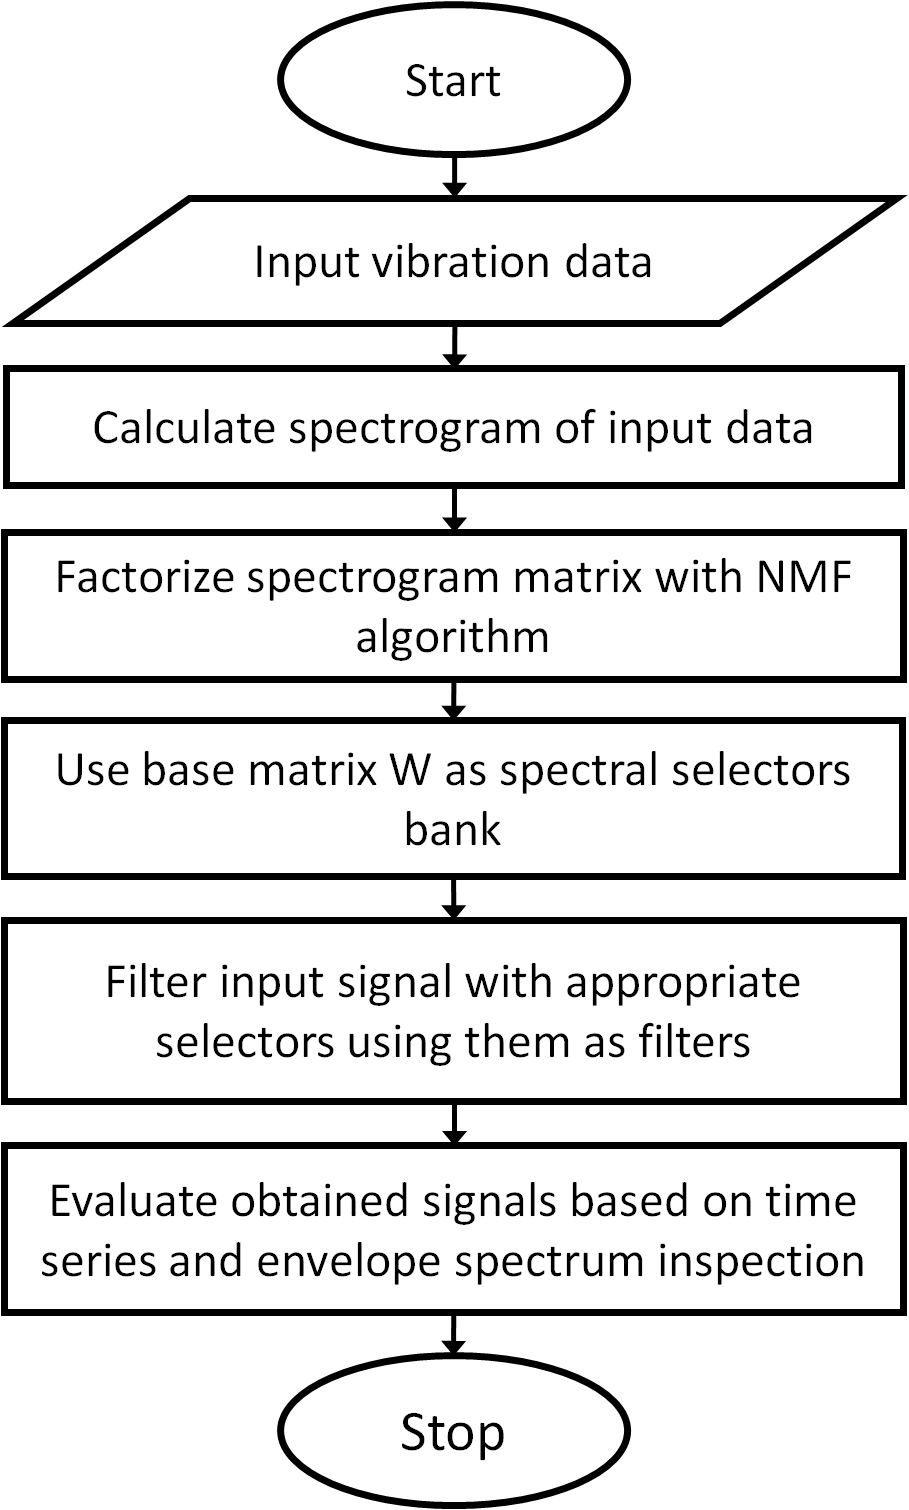
\includegraphics[width = 0.38\textwidth]{figs/block.png}
\caption{Flowchart of the diagnostic algorithm}
\label{fig: block}
\end{figure}

Functional flowchart of the proposed method is presented in Fig. \ref{fig: block}. Firstly, signal has to be transformed into a time-frequency domain. For such transformation spectrogram has been chosen, which is a square of absolute values of short-time Fourier transform (STFT), which for discrete data $x[0], x[1], ... , x[N-1]$ is given by the formula \cite{alan1989discrete}:

\begin{equation}
    \textrm{STFT}(n,k)=\sum_{m=0}^{L-1}x[n+m]w[m]e^{-j2\pi km/N},
\end{equation}
for $0\leq k \leq N-1$, and $w[.]$ is the window of length $L$. After that Nonnegative Matrix Factorization (NMF) algorithm is applied to extract spectral information about different types of processes occurring in the signal. As a result, $r$ selectors are obtained as column vectors of base matrix {\bf W}, where $r$ is the predefined expected number of processes. Finally, input signal is filtered with FFT-based FIR filter using overlap-add method, where given selector is used as filter transfer function \cite{alan1989discrete}. At the end, envelope spectra of obtained signals are calculated to inspect fundamental and harmonic frequencies of the components.

\section{Simulated data analysis}
\label{sec:sim data}
\subsection{Description of simulated data}

 In this article we analyze the simulated signal. It  consists of cyclic and noncyclic impulses. The former ones have cyclic frequency equal to 40 Hz and carrier frequency around $2500-3500$ Hz. The latter 
impulses have a center frequency equal to 5000 Hz, but
bandwidths which varies. The  MATLAB
function \emph{gauspuls}  with a center frequency $F_c = 3000$ Hz
and uniformly distributed bandwidth on
[0.2, 0.3] interval is used to reproduce the cyclic impulses. As a next step, a single impulse is replicated to obtain cyclic signal. Furthermore, in case of noncyclic impulse the same function is applied, 
however with different  centre frequency $F_c = 5000$ Hz and uniformly distributed bandwidth on [0, 1] interval. Positions of the noncyclic impulses are uniformly distributed
on the time axis. The model of the simulated signal is presented in Fig. \ref{fig:schemat sygnal}.

\begin{figure}[ht!]
    \centering
    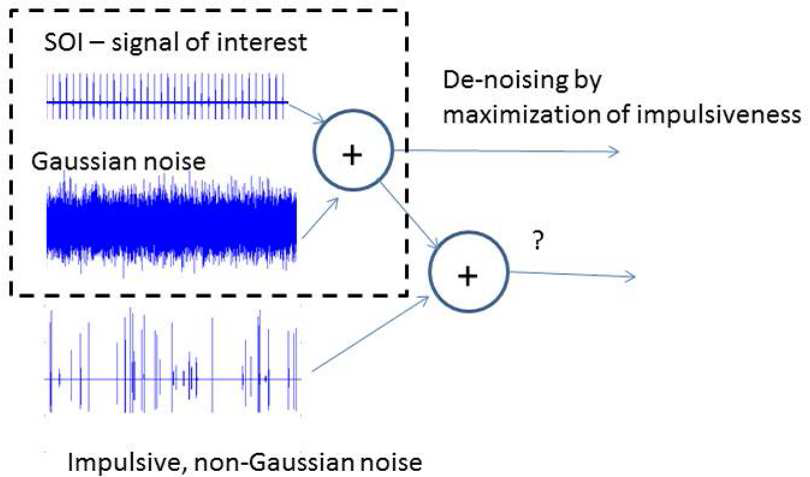
\includegraphics[width = 0.48\textwidth]{figs/schemat.png}
    \caption{The schematic model of the signal}
    \label{fig:schemat sygnal}
\end{figure}

\subsection{Results}

Time series of simulated  signal is presented in Fig. \ref{fig: input}. This data has been already addressed in \cite{wylomanskaimpulsive}, where other methods of IFB estimation have been described. Spectrogram is computed for Hamming 256-element length window where 220 samples overlap and FFT is calulated for 512 points. One can observe several strong, non-cyclic excitations emerging from the noise, but no cyclic impulses are visible. Even on spectrogram they are barely noticeable (see Fig. \ref{fig: spectrogram}).

\begin{figure}[!ht]
%\vspace{-10pt}
\centering
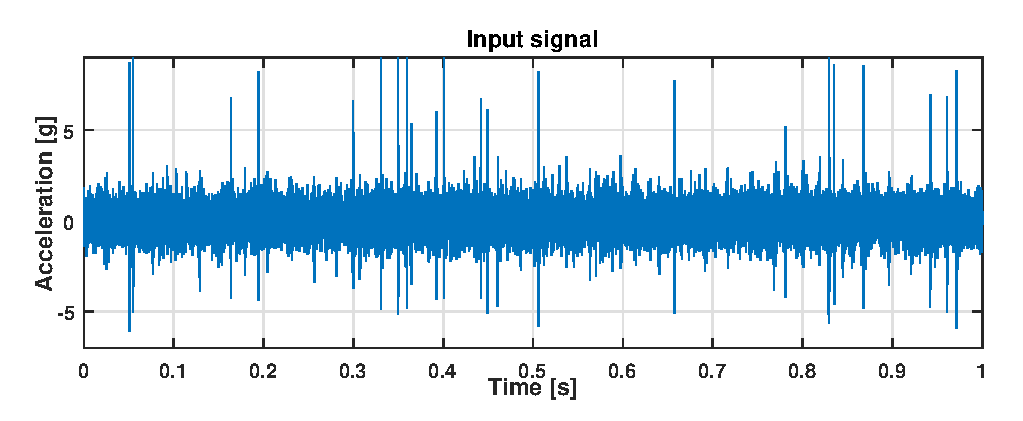
\includegraphics[width = 0.48\textwidth]{figs/input_sig.eps}
\caption{Simulated input signal}
\label{fig: input}
\end{figure}

\begin{figure}[!ht]
\centering
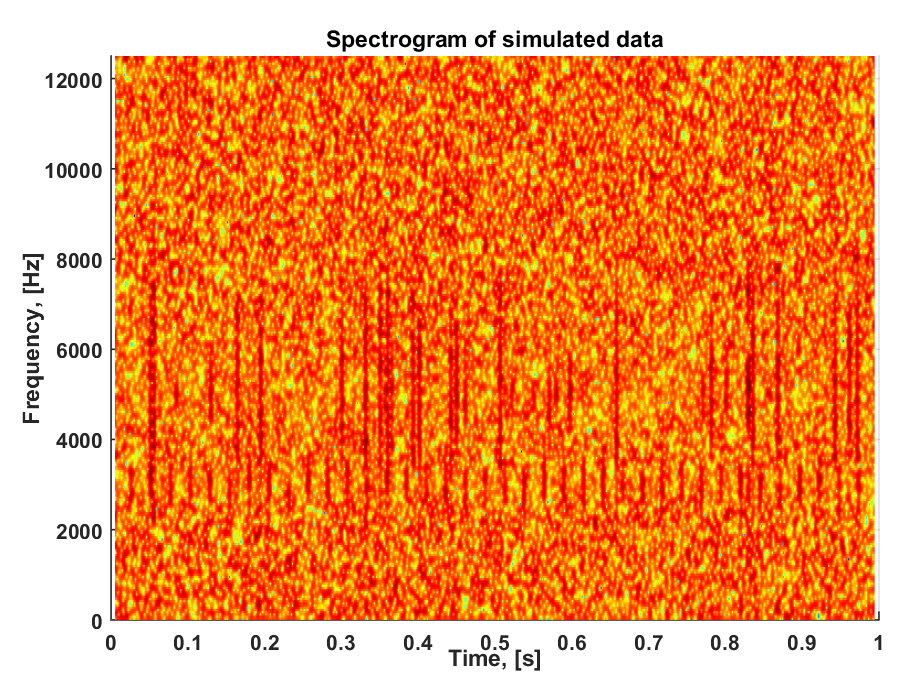
\includegraphics[width = 0.48\textwidth]{figs/input_spec.eps}
\caption{Time-frequency representation of the input signal}
\label{fig: spectrogram}
\end{figure}

As a next step, NMF algorithm differentiates spectral profiles of previously described processes (see Fig. \ref{fig: selmat}). Based on the visual inspection of the spectrogram matrix, one can recognise that second cluster describes spectrum of cyclic impulsive component, and third component is responsible for the non-cyclic process.

\begin{figure}[!ht]
\centering
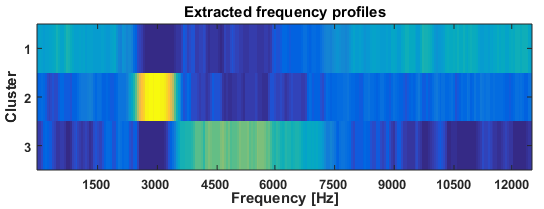
\includegraphics[width = 0.48\textwidth]{figs/selector_matrix.png}
\caption{Matrix of IFB selectors obtained by NMF}
\label{fig: selmat}
\end{figure}

Selectors used as transfer functions for the filtration step are presented in Fig. \ref{fig: selplots}. 

\begin{figure}[!ht]
\centering
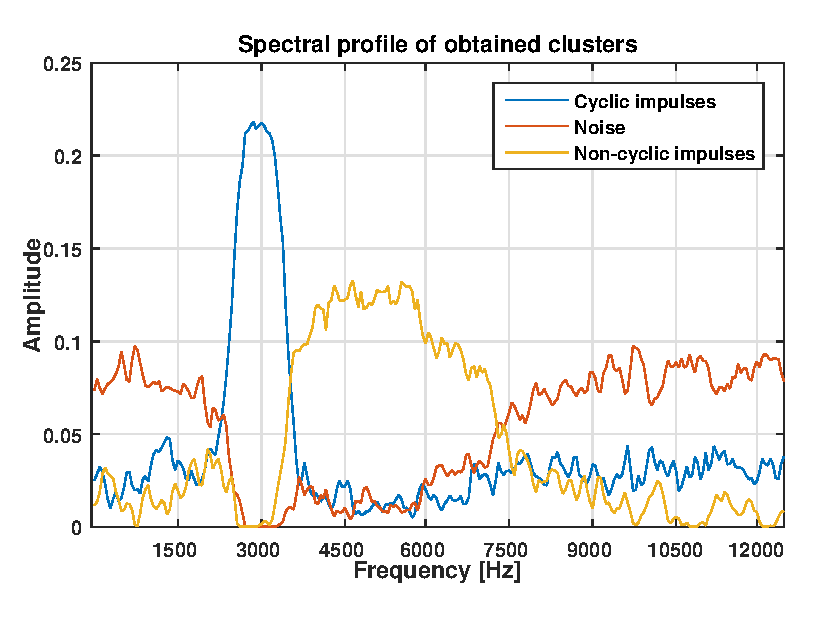
\includegraphics[width = 0.48\textwidth]{figs/selector_plot.eps}
\caption{Plot of IFB selectors for three components}
\label{fig: selplots}
\end{figure}

Input signal (Fig. \ref{fig: outplots} a) has been filtered with two selectors extracting non-cyclic and cyclic components (Fig. \ref{fig: outplots} b and c respectively). Obtained signals carry information about random impacts being natural behavior of this type of machines, and cyclic impulsive process that denotes detected local damage.

\begin{figure}[!ht]
\centering
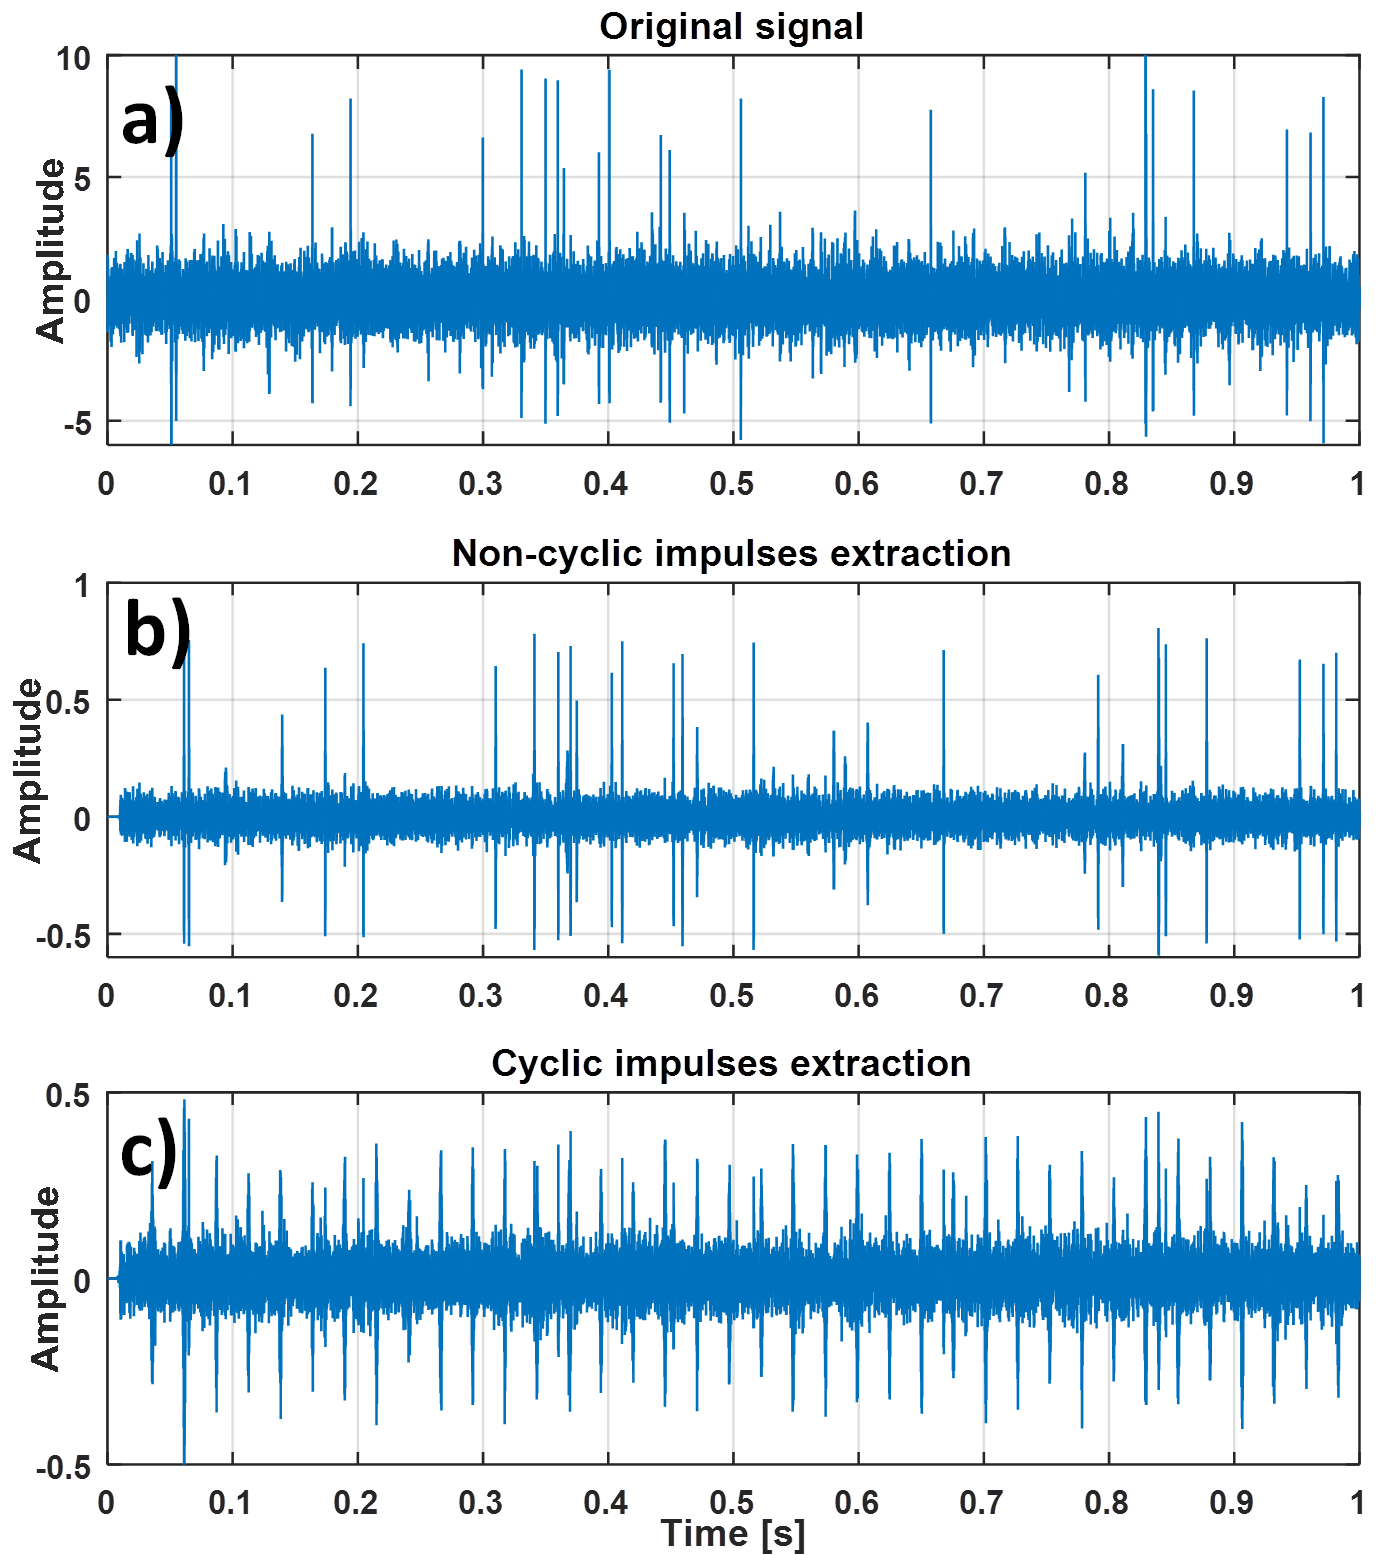
\includegraphics[width = 0.48\textwidth]{figs/output_plots.png}
\caption{Results of filtration: a) original signal, b) non-cyclic impulses, c) cyclic impulses}
\label{fig: outplots}
\end{figure}

\begin{figure}[!ht]
\centering
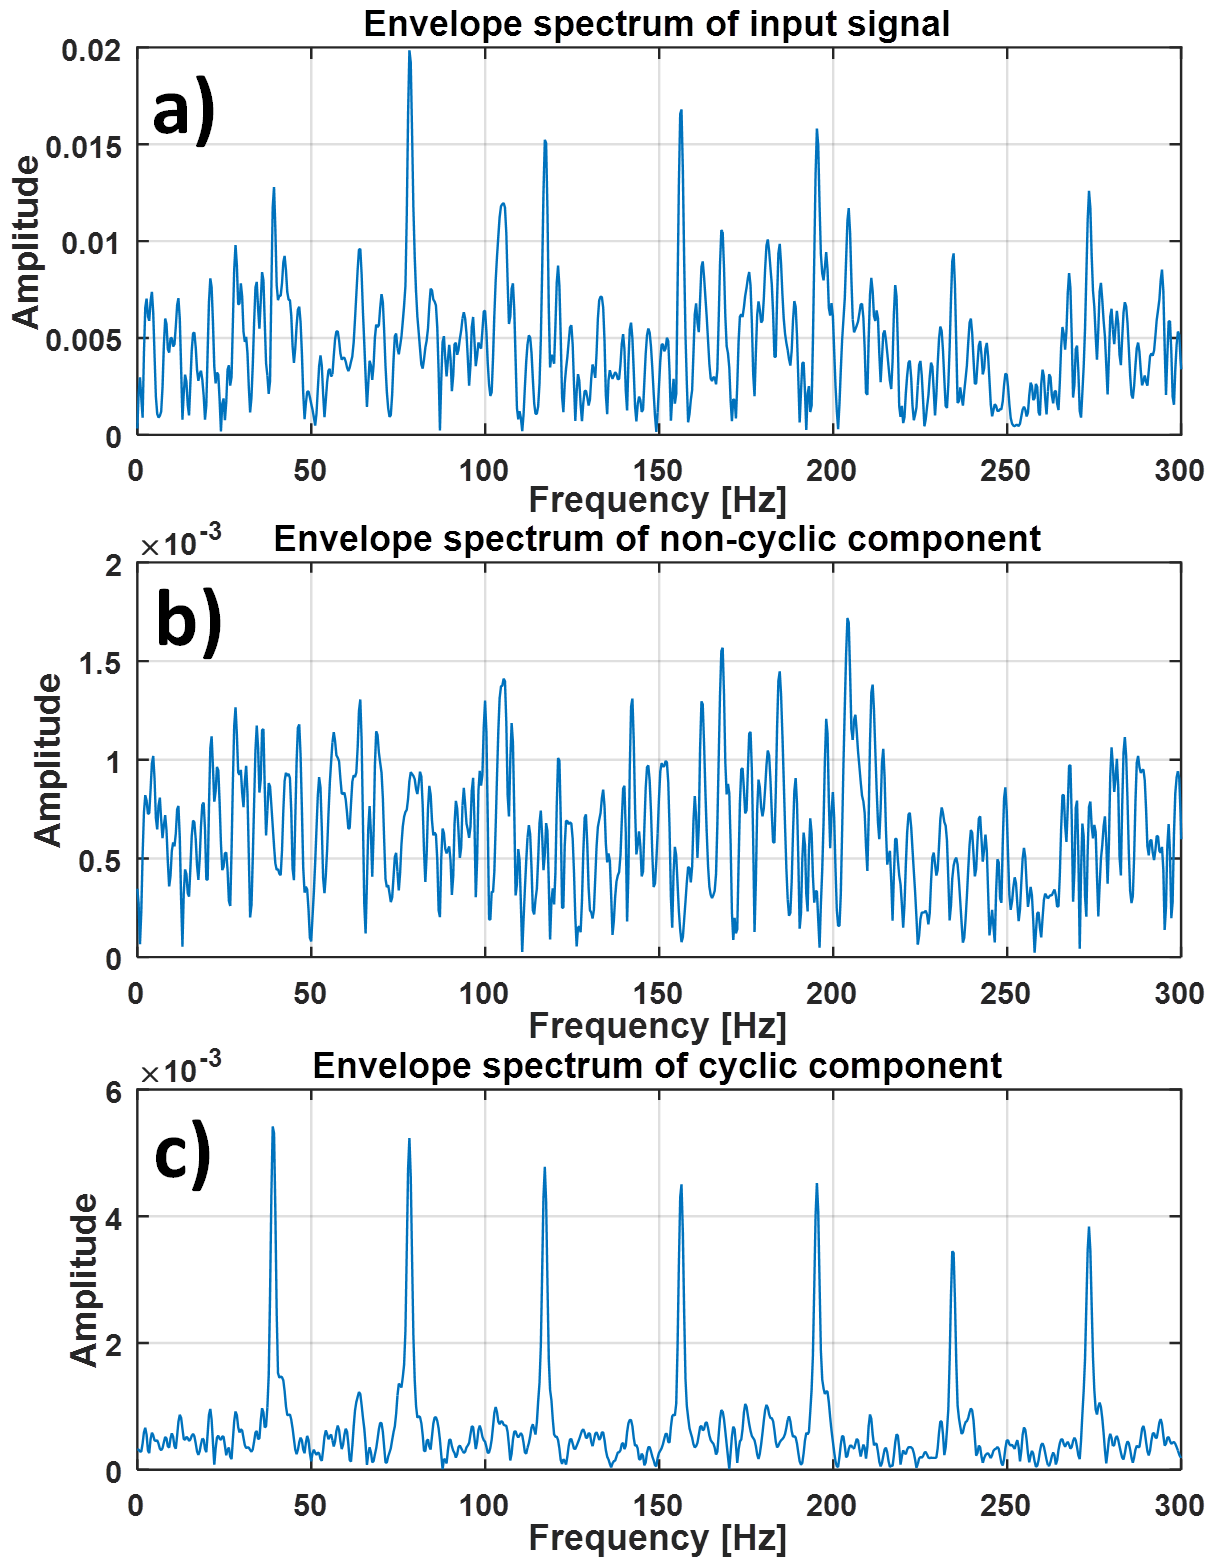
\includegraphics[width = 0.48\textwidth]{figs/output_specs2.png}
\caption{Envelope spectra of the results: a) original signal, b) non-cyclic impulses, c) cyclic impulses}
\label{fig: outspecs}
\end{figure}

In addition, quality and clarity of obtained components can be evaluated using envelope spectra (see Fig. \ref{fig: outspecs}). Spectrum of input signal (panel a) provides no conclusive information about the damage. Although there are several visible peaks in the spectrum, their presence and meaning is questionable. Envelope spectrum of non-cyclic component (panel b) looks random, which is expected effect because of randomness of impulses' bandwith and position in time domain. Finally, envelope spectrum of cyclic component (panel c) provides unquestionable series of peaks at fundamental and harmonic frequencies related to local damage (in this case 40 Hz and its multiples). 
% An example of a floating figure using the graphicx package.
% Note that \label must occur AFTER (or within) \caption.
% For figures, \caption should occur after the \includegraphics.
% Note that IEEEtran v1.7 and later has special internal code that
% is designed to preserve the operation of \label within \caption
% even when the captionsoff option is in effect. However, because
% of issues like this, it may be the safest practice to put all your
% \label just after \caption rather than within \caption{}.
%
% Reminder: the "draftcls" or "draftclsnofoot", not "draft", class
% option should be used if it is desired that the figures are to be
% displayed while in draft mode.
%
%\begin{figure}[!t]
%\centering
%\includegraphics[width=2.5in]{myfigure}
% where an .eps filename suffix will be assumed under latex, 
% and a .pdf suffix will be assumed for pdflatex; or what has been declared
% via \DeclareGraphicsExtensions.
%\caption{Simulation results for the network.}
%\label{fig_sim}
%\end{figure}

% Note that the IEEE typically puts floats only at the top, even when this
% results in a large percentage of a column being occupied by floats.


% An example of a double column floating figure using two subfigures.
% (The subfig.sty package must be loaded for this to work.)
% The subfigure \label commands are set within each subfloat command,
% and the \label for the overall figure must come after \caption.
% \hfil is used as a separator to get equal spacing.
% Watch out that the combined width of all the subfigures on a 
% line do not exceed the text width or a line break will occur.
%
%\begin{figure*}[!t]
%\centering
%\subfloat[Case I]{\includegraphics[width=2.5in]{box}%
%\label{fig_first_case}}
%\hfil
%\subfloat[Case II]{\includegraphics[width=2.5in]{box}%
%\label{fig_second_case}}
%\caption{Simulation results for the network.}
%\label{fig_sim}
%\end{figure*}
%
% Note that often IEEE papers with subfigures do not employ subfigure
% captions (using the optional argument to \subfloat[]), but instead will
% reference/describe all of them (a), (b), etc., within the main caption.
% Be aware that for subfig.sty to generate the (a), (b), etc., subfigure
% labels, the optional argument to \subfloat must be present. If a
% subcaption is not desired, just leave its contents blank,
% e.g., \subfloat[].


% An example of a floating table. Note that, for IEEE style tables, the
% \caption command should come BEFORE the table and, given that table
% captions serve much like titles, are usually capitalized except for words
% such as a, an, and, as, at, but, by, for, in, nor, of, on, or, the, to
% and up, which are usually not capitalized unless they are the first or
% last word of the caption. Table text will default to \footnotesize as
% the IEEE normally uses this smaller font for tables.
% The \label must come after \caption as always.
%
%\begin{table}[!t]
%% increase table row spacing, adjust to taste
%\renewcommand{\arraystretch}{1.3}
% if using array.sty, it might be a good idea to tweak the value of
% \extrarowheight as needed to properly center the text within the cells
%\caption{An Example of a Table}
%\label{table_example}
%\centering
%% Some packages, such as MDW tools, offer better commands for making tables
%% than the plain LaTeX2e tabular which is used here.
%\begin{tabular}{|c||c|}
%\hline
%One & Two\\
%\hline
%Three & Four\\
%\hline
%\end{tabular}
%\end{table}


% Note that the IEEE does not put floats in the very first column
% - or typically anywhere on the first page for that matter. Also,
% in-text middle ("here") positioning is typically not used, but it
% is allowed and encouraged for Computer Society conferences (but
% not Computer Society journals). Most IEEE journals/conferences use
% top floats exclusively. 
% Note that, LaTeX2e, unlike IEEE journals/conferences, places
% footnotes above bottom floats. This can be corrected via the
% \fnbelowfloat command of the stfloats package.




\section{Conclusion}
In this paper authors propose a novel approach to local damage detection in rotating machinery. Although the idea of selectors is widely known, it is proposed to perform Nonnegative Matrix Factorization of the spectrogram matrix and use base matrix as a selector bank. Analyzed data filtered with obtained selectors reveal the underlying component processes occurring in the signal, most important being the cyclic impulsive component related to local damage. Differentiation of spectral structure allows to properly distinguish particular classes of existing processes.




% conference papers do not normally have an appendix


% use section* for acknowledgment
\section*{Acknowledgment}
This work is partially (J. Wodecki, P. Kruczek, A. Wy{\l}oma{\'n}ska) supported by the Framework Programme for Research and Innovation Horizon 2020 under grant agreement n. 636834 (DISIRE -Integrated Process Control based on Distributed In-Situ Sensors into Raw Material and Energy Feedstock) 

The work is supported by the Statutory Grant no.0401/0166/16 (Rados{\l}aw Zimroz)


\bibliographystyle{IEEEtran}
\bibliography{mybib}



% that's all folks
\end{document}


% \begin{figure}[ht!]
% \vspace{-10pt}
% \centering
% \includegraphics[width = 1\textwidth]{Wykresy/L222_55_data.png}
% \caption{Real temperature data from belt conveyor gearbox after pre-processing.}
% \label{fig: L222_55_data}
% \vspace{-10pt}
% \end{figure}